\chapter{Introduction}
\inspirationalquote{
\begin{tabular}{p{0.7\textwidth}}
Please hold on. This thesis will be departing shortly for the Landslide terminal, baggage claim, ground transportation, and ticketing.
\end{tabular}}
{Pittsburgh International Airport (paraphrased)}

\subsection{Motivation}

Modern computer architectures have turned to increasing CPU core count, rather than clock speed, to improve processing power \cite{mooreslaw}.
To take advantage of multiple cores for performance, programmers must write software to execute {\em concurrently} --
using multiple {\em threads} which execute multiple parts of a program's logic simultaneously.
However, when threads access the same shared data, they may interleave in unexpected ways which change the outcome of their execution.
When an unexpected interleaving produces undesirable program behaviour,
for example, by corrupting shared data structures,
we call it a {\em concurrency bug}.
Concurrency bugs are notoriously hard for programmers to find and debug
because the specific thread interleaving required to trigger them arises at random during normal execution,
and often with very low probability.
%Concurrency bugs are notoriously hard to find and reproduce because they only appear in specific thread interleavings, which arise at random during normal program execution.
% TODO(LAYMAN): give example of trying to open car door at same time as friend turns key to unlock it.

Most commonly, a programmer searches for concurrency bugs in her code by running it many times (in parallel, in serial, or both),
hoping that eventually, it will run according to the particular interleaving required to expose a hypothetical bug.
This technique, known as {\em stress testing}, is unreliable,
providing no guarantee of finding the failing interleaving in any finite amount of time.
It also provides no assurance of correctness:
when finished, there is no way of knowing how many distinct thread interleavings were actually tested.
Nevertheless, stress testing remains popular because of how easily a programmer can use it:
she simply wraps her program in a loop, sets it to run overnight, and kills it if her patience runs out before it finds a bug.

{\em Stateless model checking} \cite{verisoft} is an alternative way to test for concurrency bugs,
or to verify their absence,
which provides more reliable coverage, progress, and verification than stress testing.
A stateless model checker tests a program by forcing it to execute a new unique thread interleaving on each iteration of the test,
capturing and controlling the randomness in a finite state space of all possible interleavings.

Unfortunately, the size of these state spaces is exponentially proportional to the size of the tested program.
% TODO(LAYMAN): explain exponential explosion by relating the parable of grains of rice on a chessboard.
For even moderately-sized programs, there may be more possible ways to interleave every thread's every instruction
than particles in the universe.
Accordingly, a programmer who wants her test to make reasonable progress through the state space must choose a subset of ways that her threads could interleave,
focusing on fully testing that subset, while ignoring other possibilities she doesn't care about.
However, it is difficult to choose a subset of thread interleavings that will produce a meaningful, yet feasible test.
Until computers can automatically navigate this trade-off in some intelligent way,
programmers will continue to fall back to the random approach of stress testing.

Another problem stateless model checking suffers is that certain types of programs cannot be tested without the programmer putting forth some manual instrumentation effort.
For example, operating system kernels implement their own sources of concurrency and their own synchronization primitives,
so the checker needs to be told how to identify and control the execution of each thread.
Some expert concurrency research wizards may be willing to add manual annotations to their code,
but required manual effort is a serious downside for anyone with a looming deadline,
and especially so for students who are still learning basic concurrency principles.
%We should not expect programmers to add effortful manual annotations to their code,
%or they will abandon our fancy technique to instead simply run stress tests until their deadline tomorrow evening.

\subsection{Contribution}

This thesis will solve both problems discussed above.
My thesis statement is as follows:

\vspace{1em}

\begin{center}
	% TODO: this sux, fix it
	{\em Thanks to the new algorithms, heuristics, and concurrency models I have developed,
	stateless model checking is an appropriate and accessible concurrency testing technique
	for programmers in both educational and real-world settings.}
\end{center}

\vspace{1em}

I have built Landslide \cite{landslide}, a stateless model checker for thread libraries and kernels,
and I have developed some techniques for automatically choosing the best thread interleavings to test
and for automatically instrumenting operating system kernels in an educational setting.
This thesis will comprise three major contributions:

\begin{enumerate}
	\item {\bf Meaningful state spaces (Chapter \ref{chap:quicksand}).}
		I will present {\em Iterative Deepening}, a new algorithm for navigating the trade-off in how many preemption points to test at once.
		Iterative Deepening incorporates state space estimation \cite{estimation} to decide on-the-fly whether each state space is worth pursuing, and uses data race analysis \cite{tsan} to find new preemption point candidates based on a program's dynamic behaviour.
		This section will include a large evaluation of the technique, comparing its performance to three prior work approaches across 600+ unique tests.
		I will show that Iterative Deepening of preemption points outperforms prior work in terms both of finding bugs quickly and of completely verifying correctness when no bug exists.
	\item {\bf Educational use (Chapter \ref{chap:education}).}
		For the past five semesters, I have offered a fully-automated version of Landslide to students in 15-410, CMU's undergraduate Operating System Design and Implementation class \cite{kspec,thrlib}, for use as a debugging aid during the thread library project.
		Recently I have also extended Landslide to handle Pintos kernel projects from other universities \cite{pintos}.
		In the two most recent semesters, I collaborated with Operating Systems course staff at two such schools, the University of Chicago and University of California at Berkeley,
		to provide debugging feedback to their students.

		At all three universities I then collected statistics on the numbers and types of bugs found,
		and surveyed students to understand the human experience,
		This section will present the study's results
		to evaluate the suitability of stateless model checking in an educational setting.
	\item {\bf Transactional Memory (Chapter \ref{chap:tm}).}
		Transactional Memory (TM) is a relatively new concurrent programming technique \cite{transactional-memory}
		which is not yet addressed by modern model checkers.
		I have extended Landslide's concurrency model to support both hardware (HTM) and software (STM) variants of TM,
		and tested several ``real-world'' TM programs and benchmarks.
		This section will discuss the theoretical techniques I used to model the new form of concurrency,
		present associated correctness proofs of my approach,
		and show the testing results.
\end{enumerate}

\subsection{Organization}

The rest of this dissertation is organized as follows.

\begin{itemize}
	\item {\bf Background:} Chapter~\ref{chap:background} will present the requisite background material on concurrent programming, stateless model checking, and the various types of programs targeted by Landslide.
	\item {\bf Landslide:} Chapter~\ref{chap:landslide} explains the design and implementation of Landslide
		%the core of my stateless model checking framework,
		and all the special features it's been equipped with over the years.
	\item {\bf Quicksand:} Chapter~\ref{chap:quicksand} presents the Iterative Deepening framework which more intelligently chooses which state spaces to test, corresponding to contribution 1 above.
	\item {\bf Education:} Chapter~\ref{chap:education} discusses my evaluation of Landslide
		in CMU's 15-410 class environment using the Pebbles kernel,
		and in the University of Chicago's and Berkeley's OS class environments using the Pintos kernel,
		corresponding to contribution 2 above.
	%\item {\bf Pebbles:} Chapter~\ref{chap:410} discusses my evaluation of Landslide in CMU's 15-410 class environment using the Pebbles kernel, corresponding to contribution 2 above.
	%\item {\bf Pintos:} Chapter~\ref{chap:410} discusses my evaluation of Landslide in the University of Chicago's and Berkeley's OS class environments using the Pintos kernel, corresponding to contribution 2 above.
	\item {\bf Transactional Memory:} Chapter~\ref{chap:tm} presents my extension of Landslide's concurrency model to handle transactional concurrency and the evaluation thereof, corresponding to contribution 3 above.
	\item {\bf Related Work:} Chapter~\ref{chap:relatedwork} honors my neighbours and ancestors in research spirit.
	\item {\bf Conclusion:} Chapter~\ref{chap:conclusion} provides some thoughts on the future of the field.
\end{itemize}

\newpage
\thispagestyle{empty}
\begin{center}
\begin{tabular}{c}
\vspace{12em} \\
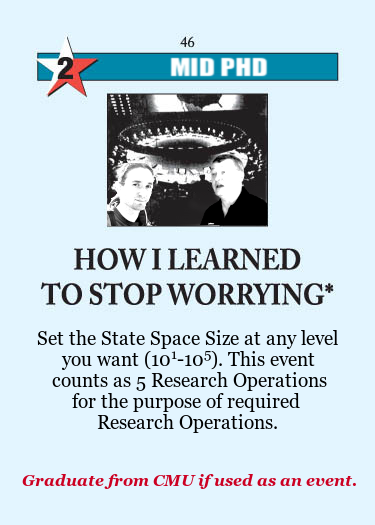
\includegraphics[width=0.55\textwidth]{how-i-learned.png}
\end{tabular}
\end{center}
